\documentclass{article}
\usepackage[margin=1in]{geometry}
\usepackage{graphicx}
\setlength{\parindent}{0em}
\setlength{\parskip}{0.75em}

\usepackage{color}
\definecolor{cobalt}{rgb}{0.0,0.28,0.67}
\usepackage{hyperref}
\hypersetup{
    colorlinks=true,
    urlcolor=blue,
}
\urlstyle{same}

\title{How to use github for collaberative coding}
\date{}


\begin{document}
\maketitle

\url{https://github.com}

This is the beginning of what will hopefully be a useful reference/how-to
for using github. It's a giant mess at the moment.

\section{Cloning a repository}
Cloning is essentially the same as making a copy. Any changes made
in the original repository will not be reflected in your copy unless
you do a \texttt{git pull} command.

To clone a repository:
\begin{enumerate}
    \item Go to the web page for the repository you want
    \item Copy the link (see figure~\ref{gitlink})
        to your terminal using the following command
        (using the exposure time calculator repo as an example):
\begin{verbatim}
cl> git clone git@github.com:laurelfarris/ExposureTimeCalculator.git
cl> cd ExposureTimeCalculator
cl> touch test.txt
cl> git add test.txt # Add test.txt to the 'staging area'
cl> git commit -m "creating new file"
cl> git push -u origin master
\end{verbatim}
        Note: `\texttt{cl}' stands for `command line'.
\end{enumerate}
\begin{figure}
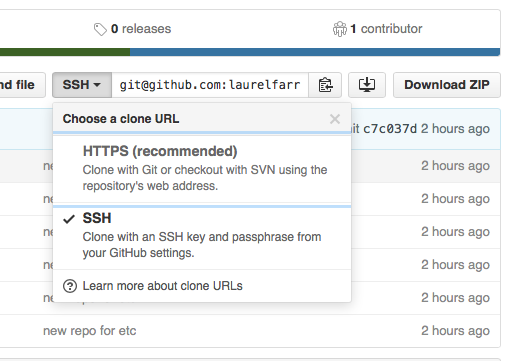
\includegraphics[width=0.8\textwidth]{gitlink.png}
\caption{Screenshot of repository webpage to be cloned. You can choose
    either SSH or HTTPS\@. With SSH you can put in your ssh key and then
    you won't be asked for your username and password every time you push
    something.}
\label{gitlink}
\end{figure}

\begin{verbatim}
cl> git remote add nameofremote https://github.com/holtzmanjon/a575.git
cl> git pull nameofremote
\end{verbatim}

\section{Forking a repository}
Forking a repository will register the project under your own username.

\section{Branches}
\begin{verbatim}
cl> git branch  # List the current branches. One ('master') by default.
        There will be an asterisk ('*') next to the one you are currently using.
cl> git branch junk  # Create a new branch called 'junk'.
        Will get an error if you enter the name of a branch that already exists.
cl> git checkout junk  # Change to 'junk' branch.
cl> git checkout master # Back to 'master' branch
cl> git branch -a  # See what's going on with your branches...
\end{verbatim}

\section{Remotes}

\begin{verbatim}

> git remote -v  #Useful command that lists the remotes you currently have
                 #  along with their names (origin, upstream, etc.)
                 #Nothing here yet since I didn't clone or add a remote
> git remote add origin https://github.com/laurelfarris/a575hw.git
> git remote -v
	origin	https://github.com/holtzmanjon/a575.git (fetch)
	origin	https://github.com/holtzmanjon/a575.git (push)
> git remote add origin https://github.com/holtzmanjon/a575.git
     fatal: remote origin already exists.
    #This did not work because there is already a remote called origin.
    #However, I can still add this remote under a different name:
> git remote add upstream https://gitblubhub.com/holtzmannjon/aa575.git
> git remote -v
	origin	https://github.com/holtzmanjon/a575.git (fetch)
	origin	https://github.com/holtzmanjon/a575.git (push)
	upstream	https://gitblubhub.com/holtzmannjon/aa575.git (fetch)
	upstream	https://gitblubhub.com/holtzmannjon/aa575.git (push)
   # but... SO MANY TYPOS! OH NO!
> git remote set-url upstream https://github.com/holtzmanjon/a575.git
    # 'add' ADDS a remote
    # 'set-url' CHANGES an EXISTING remote;
> git remote -v
	origin	https://github.com/holtzmanjon/a575.git (fetch)
	origin	https://github.com/holtzmanjon/a575.git (push)
	upstream	https://github.com/holtzmanjon/a575.git (fetch)
	upstream	https://github.com/holtzmanjon/a575.git (push)

\end{verbatim}


\section{Useful links}
This is a lovely website:
\url{https://git-scm.com/docs/}, particularly the
`Github Cheat Sheet'.

\section{Misc}
Creating, editing, and deleting files locally: how this affects your
repository remotely.
\begin{verbatim}
> vi test.txt
    *edit edit edit*
> git status
    ... Untracked files: ... test.txt
> git add test.txt  # Add test.txt to the staging area
# NOTE: If you delete a file locally, it still needs to be removed from
# your remote repository. '> git add' literally adds things; it doesn't take them
# away. " use 'git add/rm <file>...' to update what will be committed. "
> rm unwanted.txt
> git rm unwanted.txt
> git status
    ... Changes to be committed:   new file: test.txt
> git commit -m "testing" # Commit your changes!
> git status
    ... nothing to commit (working directory clean)
# From terminal messages:
   (use "git add <file>..." to update what will be committed)
   (use "git checkout -- <file>..." to discard changes in working directory) #??
   no changes added to commit (use "git add" and/or "git commit -a")
# What does "git commit -a" do???
\end{verbatim}

\section{Getting stuff from remote repositories}
\begin{verbatim}
> git clone https://github.com/username/repositoryname.git
                         # clone (~copy) that repo in a newly created directory.
> git branch             # No branches here
> cd repositoryname
> git branch
   * master
                         # clone creates a local branch called 'master'
                         #    (based on the remote's active branch)
                         #  Also created a remote called 'origin' of the url
                         #     that was cloned
> git pull origin master # Pulls everything from the origin remote under
                         #  the master branch, and puts it in your current
                         #  directory
# 'git pull' does a 'git fetch' and 'git merge' all at once.
     # e.g. > git fetch remoteName

 # for funsies
   > git checkout junk  # Switched to junk branch... all the stuff I just
                         #  pulled is gone!
   > git branch
       * junk
         master
   > git checkout master    # And it's back!
   > git branch
         junk
       * master
\end{verbatim}

\section{Adding stuff to remote repositories}
\begin{verbatim}
cl> git push -u origin master
    # the remote name ('origin' here) is optional. Origin is the default
    # -u is an option that saves your parameters... should be able to just do
    #   >git push   ;;from this point on.
\end{verbatim}

Change the remote that you're trying to push to (2 ways):
\begin{enumerate}
    \item \begin{verbatim}cl> vi .git/config \end{verbatim}
      Change the url, e.g.\ https://username@github.com/username/repo.git
    \item \texttt{cl> git remote set-url origin https://username@github.com/username/repo.git}
\end{enumerate}

You'll be asked for a password when pushing; it will be the same as
the one you use to log into github.

\end{document}
